\documentclass[11pt]{article}
\usepackage[utf8]{inputenc}
\usepackage{graphicx}
\usepackage{url}
\usepackage{amsmath}
\usepackage{float}


\title{
	{Computer Vision 1 - Assignment 2 \\
	Linear Filters: Gaussians and Derivatives}
}
\author{
Selene Baez Santamaria (10985417) - Andrea Jemmett (11162929)}
\date{\today}

\begin{document}

\maketitle

\section{1D Gaussian Filter}
% Question: "Compare your function with MATLAB’s built-in fspecial. What are the
% differences?"
Our function takes the same arguments as the built-in fspecial, but it generates
different output. While our function generates a vector of size $kernelLength$,
the \emph{fspecial} function returns a rectangular or squared matrix dependant on the
$hsize$ parameter.


\section{Convolving an image with a 2D Gaussian}
% Question 1: Show that the outputs of convolution with the 2D kernel (i.e. the
% one corresponding to the two 1D kernels) and convolution with 1D kernels are
% essentially the same.  Use kernel length of 11.  Report the numerical
% equivalence as well as plots at every stage of filtering pipeline.  Question
% 2: Explain the benefits of kernel separability, shortly.
We use a value of $\sigma_x = 2$ and $\sigma_y = 2$ and a kernel length of 11
(as requested). First we call the \emph{gaussian} function defined in the
previous section to get two 1D filters, one with each $\sigma$. We multiply
those 1D vectors to obtain a 2D gaussian kernel.
To convolve the images with kernels we use the built-it function $conv2$. After
testing the different options we found out the following:

\begin{description}
	\item[full] performs the full convolution. Visually, we note that the
		produced images have black frames on the edges since the image size
		is slightly (10 pixels) larger than the original image; this is due
		to the fact that the convolution operation ``spreads'' pixel
		intensities over neighboring pixels overflooding outside the
		original image size;
	\item[same] returns the central part of the convolution, that is the image
		returned as output is of the same size of the input matrix $A$;
	\item[valid] performs convolution but omits those parts of the convolution
		that are computed not exclusively using image pixels (image edges);
		the resulting image is indeed smaller than the original.
\end{description}

In order to check that both functions produce the same images we make a pixel
per pixel numeric comparison. We check that the absolute value of the difference
among the values is less that a small value $\epsilon = e^{-12}$. Hereby we show
the original and filtered images using the \emph{same} option:

\begin{figure}[H] \centering
	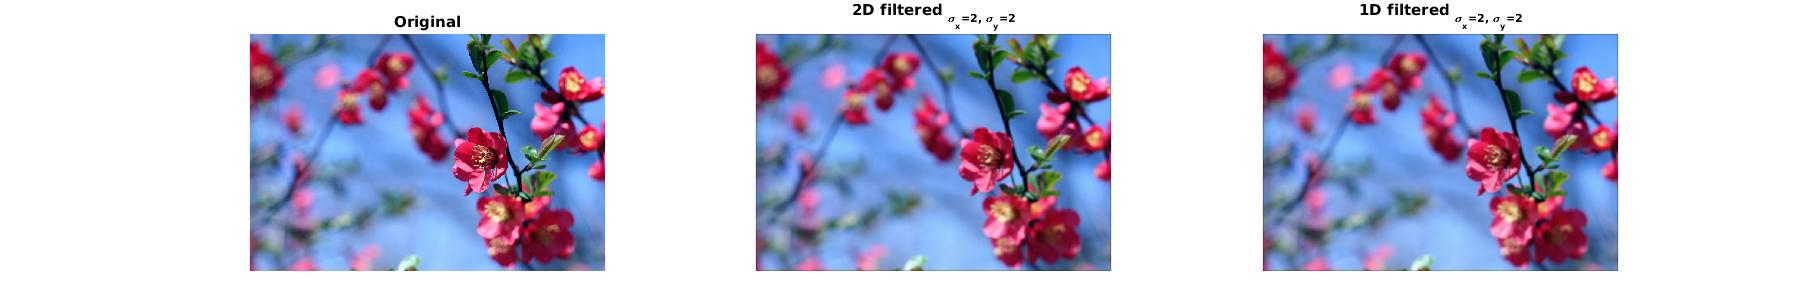
\includegraphics[width=1\textwidth]{imgs/flowers_conv.jpg}
	\caption{Comparison for flowers.jpg. From left to right: original image, image
	filtered with 2D kernel and image filtered with 1D kernel. All images have a
	$\sigma$ value of 2}
	\label{fig:flowers}
\end{figure}

\begin{figure}[H] \centering
	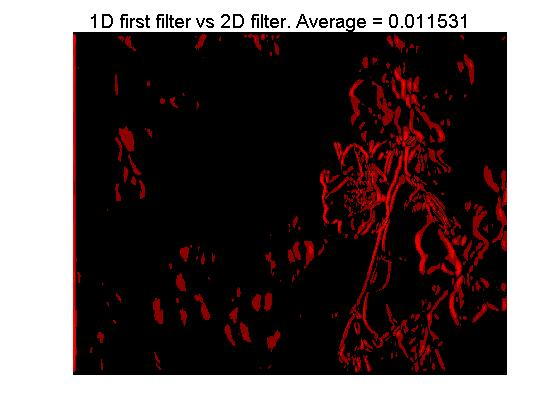
\includegraphics[width=.9\textwidth]{imgs/flowers_col_heatmap.jpg}
	\caption{Heatmap showing the absolute difference per pixel between Step
		1 of 1D filtering and 2D final filtered image for flowers.jpg. Reported
		mean error per pixel is $0.0115$}
	\label{fig:flowers_col_heatmap}
\end{figure}

\begin{figure}[H] \centering
	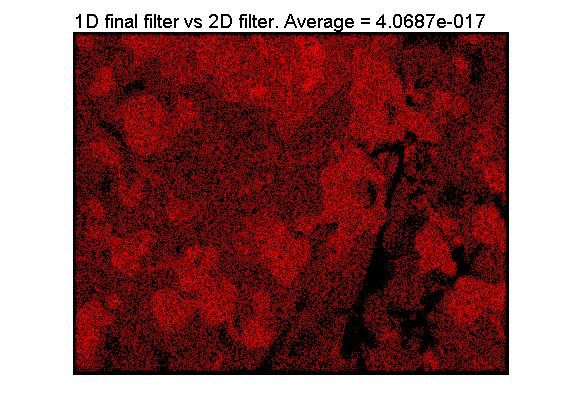
\includegraphics[width=.9\textwidth]{imgs/flowers_heatmap.jpg}
	\caption{Heatmap showing the absolute difference per pixel between both
		final filtered images for flowers.jpg. Reported mean error per pixel is
		$4.0687 e^{-17}$}
	\label{fig:flowers_heatmap}
\end{figure}

\begin{figure}[H] \centering
	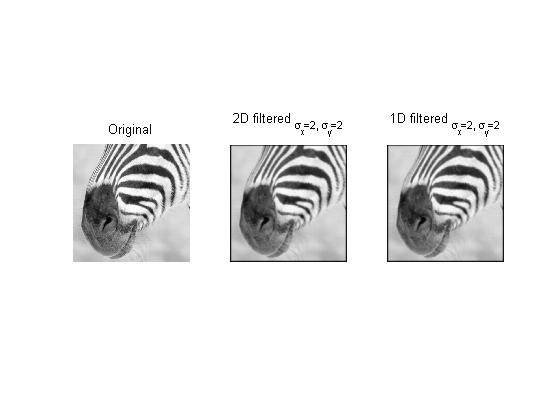
\includegraphics[width=1\textwidth]{imgs/zebra_conv.jpg}
	\caption{Comparison for zebra.png (original, 2D kernel, 1D kernel with
		$\sigma=2$). Reported mean error per pixel is $5.5609 e^{-17}$}
	\label{fig:zebra}
\end{figure}

\begin{figure}[H] \centering
	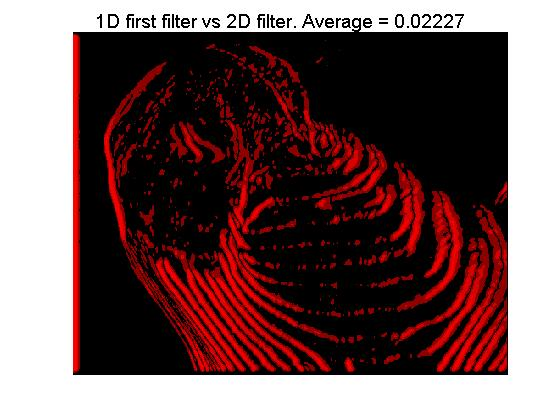
\includegraphics[width=.9\textwidth]{imgs/zebra_col_heatmap.jpg}
	\caption{Heatmap showing the absolute difference per pixel between Step
		1 of 1D filtering and 2D final filtered image for zebra.png. Reported
		mean error per pixel is $0.0223$}
	\label{fig:zebra_col_heatmap}
\end{figure}

\begin{figure}[H] \centering
	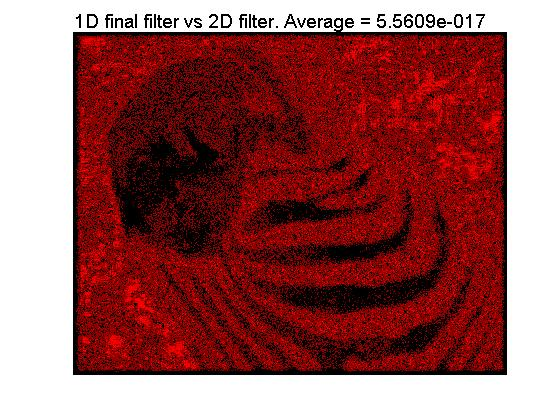
\includegraphics[width=.9\textwidth]{imgs/zebra_heatmap.jpg}
	\caption{Heatmap showing the absolute difference per pixel between both
		final filtered images for zebra.png. Reported mean error per pixel is
		$5.5609 e^{-17}$}
	\label{fig:zebra_heatmap}
\end{figure}

% We note that the 1D convoluted image takes longer to compute.
Having kernel separability is helpful since the number of operations needed to
perform the convolution operation are fewer than with a full 2D kernel. For
example filtering an M-by-N image with a P-by-Q kernel would require $MNPQ$
operations. If the kernel is separable, we can apply the convolution in an
ordered fashion, first by applying a vector kernel to columns and then filtering
the results using a vector kernel on the rows. Filtering in these two steps
requires respectively $MNP$ and $MNQ$ operations, so the total number of
operations is $MN(P + Q)$, which is less than $MNPQ$.

\section{Gaussian Derivative}
We implemented a function called $gaussianDer$ which computes the first order
derivative of a gaussian kernel. The function takes as parameters a path to the
image to filter, a gaussian kernel and a $\sigma$ value. We try this filter with
the same image with different sigma values and a kernel length of $11$. The
resulting filtered images are shown in Figure \ref{fig:zebra_deriv}.  The
Gaussian derivative may be used to find edges in am image. An application could
be countoruing an image. From the Figure it is possible to note that for values
of the standard deviation smaller than $1$ and bigger than $2$ the filter is
almost unable to detect any edge, achieving the best results with $\sigma=1.5$.

\begin{figure}[H] \centering
	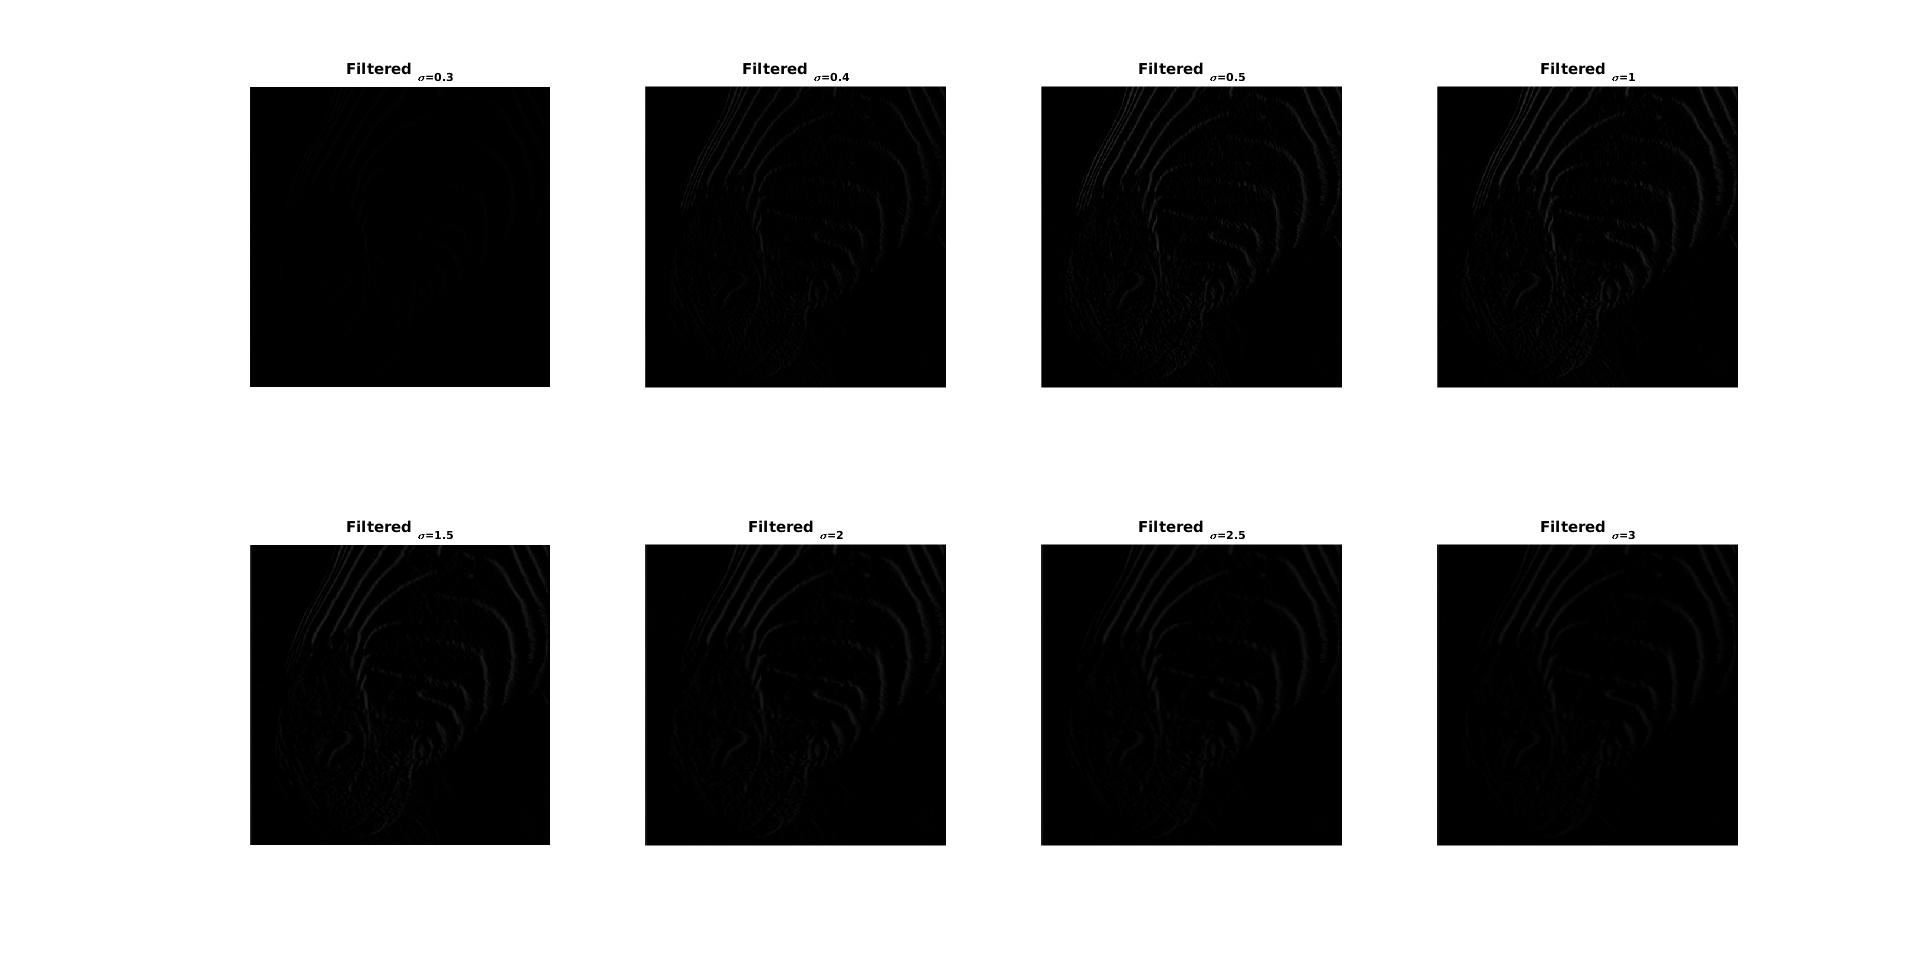
\includegraphics[width=1\textwidth]{imgs/zebra_deriv.jpg}
	\caption{Application of the first order Gaussian derivative to the Zebra
		image with different $\sigma$ values (from top left: $0.1, 0.2,
		0.3, 0.4, 0.5, 1, 1.5, 2, 2.5, 3$).}
	\label{fig:zebra_deriv}
\end{figure}

\begin{figure}[H] \centering
	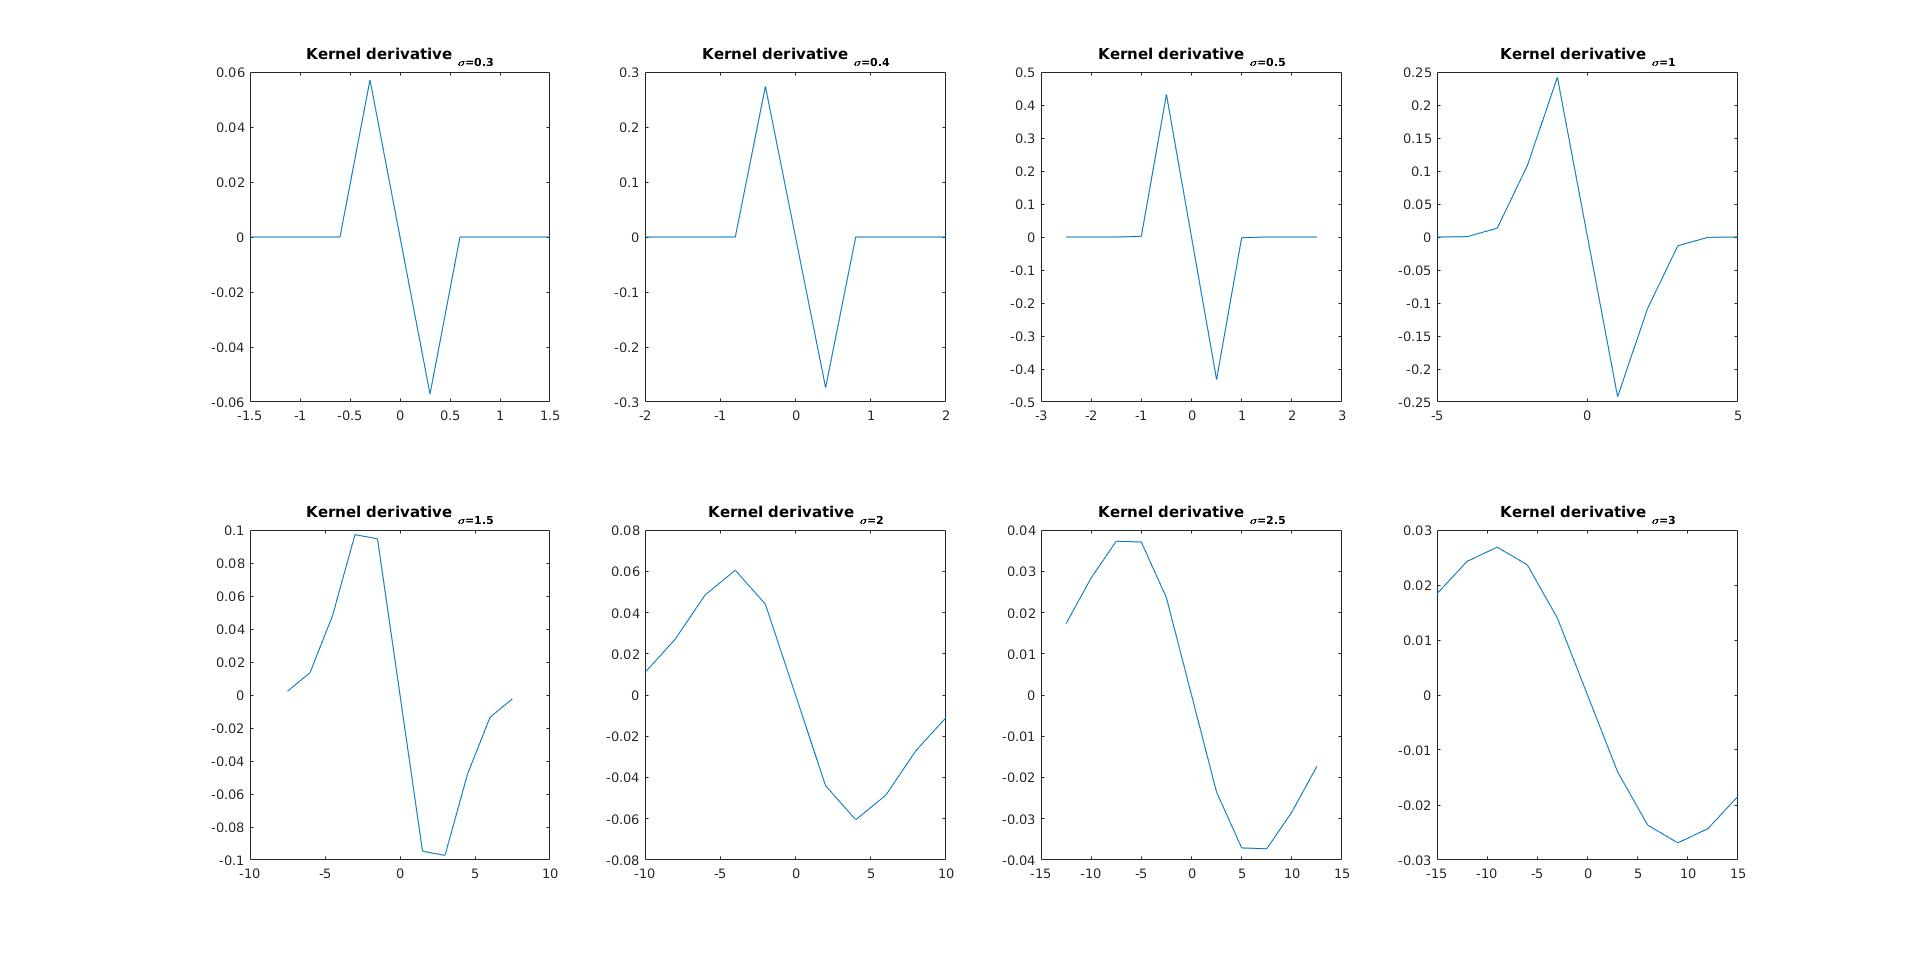
\includegraphics[width=1\textwidth]{imgs/gauss_deriv.jpg}
	\caption{First order Gaussian derivative plotted on a range in
		$[-5\sigma, 5\sigma]$}
	\label{fig:gauss_deriv}
\end{figure}

From Fig. \ref{fig:gauss_deriv} is easily noticeable how the shape of the kernel
signal affects the filtering results. For smaller sigma values the first order
Gaussian derivative is sharper and for values smaller than $1$ it is unable to
detect edges small enough. Vice versa happens with bigger values of $\sigma$ for
which the filter is unable to detect enough big edges.

\end{document}

